\documentclass{standalone}
\usepackage{tikz}
\usetikzlibrary{shapes,arrows,positioning}
\begin{document}
  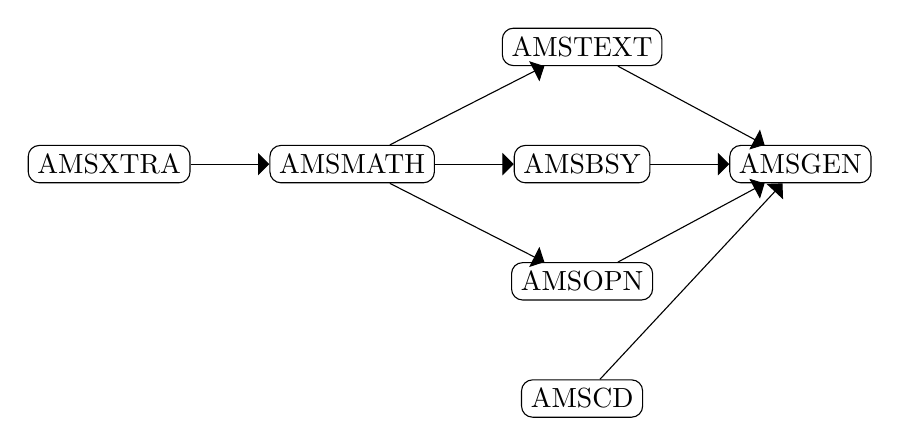
\begin{tikzpicture}
  
  \tikzset{main node/.style={rectangle, draw,
  		text centered, rounded corners}, }
  \tikzset{main verb/.style={minimum size=1cm}, }
  \tikzset{linea/.style={-triangle 90}, }
    \node[main node] (1) {AMSXTRA};
    \node[main node] (2) [right =of 1]  {AMSMATH};
    
    \node[main node] (5) [right =of 2]  {AMSBSY};
    \node[main node] (6) [below =of 5]  {AMSOPN};
    \node[main node] (4) [above =of 5]  {AMSTEXT};
    \node[main node] (3) [below =of 6] {AMSCD};
    \node[main node] (7) [right =of 5] {AMSGEN};

\foreach \x /\y in{1/2,2/4,2/5,2/6,4/7,5/7,6/7,3/7}
  \path[linea] (\x) edge node {} (\y);
%%  
\end{tikzpicture}
\end{document}